\chapter{GIỚI THIỆU, MÔ TẢ ĐỀ TÀI}

Chương 2. GIỚI THIỆU, MÔ TẢ ĐỀ TÀI

\section{Giới thiệu bài toán tổng thể}

\subsection{Bối cảnh và yêu cầu hệ thống}

Hệ thống quản lý thư viện được xây dựng nhằm đáp ứng nhu cầu số hóa toàn bộ quy trình vận hành của một thư viện hiện đại, từ khâu quản lý kho sách, cho mượn – trả sách, theo dõi độc giả cho đến thống kê báo cáo và quản lý doanh thu. Hệ thống hướng đến ba nhóm người dùng chính: Độc giả (Reader) có thể tra cứu sách, gửi yêu cầu mượn/trả, theo dõi lịch sử mượn và thanh toán phí phạt trực tuyến, Thủ thư (Librarian) quản lý phiếu mượn, xác nhận trả sách, quản lý phí phạt và doanh thu và Quản trị viên (Admin) có toàn quyền quản trị hệ thống. Để đáp ứng yêu cầu phát triển song song giữa ba nhóm sinh viên và đảm bảo tính module hóa, hệ thống được thiết kế theo kiến trúc microservices và phân tách thành ba dịch vụ độc lập. Mỗi dịch vụ vận hành trong một tiến trình riêng, có cơ sở dữ liệu riêng và giao tiếp với nhau thông qua REST API được định nghĩa rõ ràng trong API Contract. Cách tiếp cận này cho phép mỗi nhóm tự do lựa chọn công nghệ phù hợp, phát triển độc lập và triển khai riêng biệt mà không gây ảnh hưởng đến các dịch vụ khác.

\subsection{Phân chia dịch vụ}

Hệ thống được tổ chức thành ba dịch vụ chính với trách nhiệm và phạm vi được phân định rõ ràng: Dịch vụ Danh mục – Catalog Service (N1): Đây là dịch vụ nền tảng, chịu trách nhiệm quản lý toàn bộ thông tin về kho sách của thư viện. Các chức năng chính bao gồm thêm mới, cập nhật, xóa và tra cứu đầu sách, quản lý số lượng bản sao, theo dõi trạng thái sách (có thể mượn, đã mượn hết, ngừng phục vụ) và cung cấp API tìm kiếm sách theo từ khóa, thể loại hoặc tác giả. N1 đóng vai trò là nguồn dữ liệu chính xác duy nhất (single source of truth) về thông tin sách cho toàn bộ hệ thống. Các dịch vụ khác khi cần thông tin sách đều phải truy vấn qua API của N1. Dịch vụ Lưu thông – Circulation Service (N2): Đây là dịch vụ trung tâm do nhóm em phụ trách, đảm nhiệm toàn bộ nghiệp vụ lưu thông của thư viện. N2 xử lý các luồng nghiệp vụ chính như tạo phiếu mượn sách, duyệt/từ chối yêu cầu mượn, xác nhận

trả sách và kiểm tra tình trạng sách khi trả, gia hạn thời gian mượn, tính toán và quản lý phí phạt quá hạn, hư hỏng hoặc mất sách, ghi nhận doanh thu từ phí mượn sách và phí phạt, quản lý đánh giá sách từ độc giả và cung cấp dashboard thống kê cho thủ thư. N2 tương tác với N1 để kiểm tra số lượng và trạng thái sách khi xử lý mượn/trả và với N3 để xác thực người dùng và lấy thông tin độc giả. Dịch vụ Định danh – Identity Service (N3): Dịch vụ này chịu trách nhiệm quản lý tài khoản người dùng và xác thực cho toàn bộ hệ thống. N3 cung cấp API đăng nhập, đăng ký, quản lý thông tin cá nhân, phân quyền theo vai trò (Reader, Librarian, Admin) và cấp JWT token để các dịch vụ khác xác thực người dùng. N3 cũng quản lý mã thẻ thư viện (Library Card) – một định danh quan trọng được N2 sử dụng để liên kết phiếu mượn với độc giả cụ thể.

Auth validate GET /api/books

Catalog Circulation Identity Service (N1) Service (N2) Service (N3)

Token + User info Book data REST API

Client (Browser/App)

Hình 2.1 Sơ đồ tổng quan kiến trúc microservices hệ thống quản lý thư viện

\subsection{API Gateway và luồng dữ liệu}

Để che giấu sự phức tạp của kiến trúc microservices khỏi phía client, toàn bộ hệ thống sử dụng một API Gateway làm điểm truy cập duy nhất. Client (trình duyệt web hoặc ứng dụng di động) gửi tất cả yêu cầu đến Gateway, sau đó Gateway định tuyến (route) đến dịch vụ tương ứng dựa trên đường dẫn URL. Cách thiết kế này mang lại nhiều lợi ích: client không cần biết địa chỉ cụ thể của từng microservice, các vấn đề cross-origin (CORS) được giải quyết tập trung tại Gateway và có thể dễ dàng thêm các chức năng như rate limiting, logging hay caching ở tầng Gateway. Trong hệ thống triển khai thực tế, Gateway được cấu hình để định tuyến các yêu cầu có đường dẫn /api/circulation đến dịch vụ N2, /api/books đến dịch vụ N1 và

kèm nhận xét). Thủ thư có thể xem và quản lý các đánh giá này. Tính năng này được thiết kế dưới dạng embed widget để N3 có thể nhúng vào giao diện của mình. Giao diện người dùng kép: N2 cung cấp hai giao diện riêng biệt cho hai nhóm người dùng. Giao diện Độc giả (Reader UI) được xây dựng bằng Vue 3 + Vuetify, cung cấp trải nghiệm duyệt sách, quản lý giỏ mượn và theo dõi lịch sử. Giao diện Thủ thư (Librarian UI) được xây dựng bằng Vue 3 + Ant Design Vue, cung cấp dashboard thống kê và các công cụ quản lý nghiệp vụ chuyên sâu.

\subsection{Kiến trúc dịch vụ N2}

Tầng Trình bày (Presentation)

Reader UI Librarian UI Embed Widgets Swagger UI (Vue 3 + Vuetify) (Vue 3 + Ant Design) (iframe)

HTTP/JSON Tầng API (REST Controllers)

Circulation Books Favorites Users Controller Controller Controller Controller

Tầng Nghiệp vụ (Business Logic) JWT Auth Middleware Policy Engine N1/N3 HTTP Clients Event Publisher

Tầng Dữ liệu (Data)

SQL Server / SQLite N1 Catalog N3 Identity (Entity Framework) (HTTP Client) (HTTP Client)

Hình 2.2 Sơ đồ kiến trúc phân tầng của Circulation Service (N2)

/api/Auth/validate để kiểm tra trạng thái tài khoản còn active không và cuối cùng, sau khi token hợp lệ, các thuộc tính [Authorize] và [Authorize(Roles = "Librarian,Admin")] trên controller kiểm tra quyền truy cập dựa trên role claim trong token. Việc xác thực bổ sung với N3 đảm bảo rằng ngay cả khi token chưa hết hạn, nếu tài khoản đã bị vô hiệu hóa, yêu cầu vẫn bị từ chối. Middleware này được đặt trước app.UseAuthorization() trong pipeline và áp dụng cho tất cả các request có đường dẫn /api/.

Luồng xử lý mượn sách

Luồng mượn sách là nghiệp vụ phức tạp nhất của N2, được triển khai trong phương thức BorrowAsync() của CirculationController, với các bước xử lý như sau: Bước 1 – Kiểm tra quyền truy cập: Hệ thống xác minh rằng người dùng hiện tại có quyền thao tác trên mã thẻ (CardNumber) được chỉ định. Nếu không, trả về HTTP 403 Forbidden. Bước 2 – Xác thực dữ liệu đầu vào: Kiểm tra các trường bắt buộc (BookId, UserId, CardNumber) và tính hợp lệ của ngày mượn/ngày hết hạn. Bước 3 – Tra cứu sách từ N1: N2 gọi API của N1 để lấy thông tin sách và kiểm tra số lượng còn lại. Nếu sách không tồn tại hoặc đã hết, trả về lỗi tương ứng. Bước 4 – Kiểm tra giới hạn mượn: Đếm số sách đang mượn của độc giả và đối chiếu với giới hạn hàng tháng (mặc định 5 cuốn). Nếu vượt quá, từ chối yêu cầu. Bước 5 – Tạo phiếu mượn: Tạo một hoặc nhiều bản ghi BorrowTransaction (tùy theo số lượng sách yêu cầu) với trạng thái “Pending”. Bước 6 – Phát sự kiện: Ghi các event vào bảng PublishedEventLogs để N3 có thể đồng bộ trạng thái: sự kiện borrow.requested (yêu cầu mượn) và book.availability.changed (thay đổi số lượng sách khả dụng). Bước 7 – Lưu và phản hồi: Lưu tất cả thay đổi vào cơ sở dữ liệu trong một transaction và trả về thông tin phiếu mượn cho client.

\paragraph{Cơ chế Event Logging}

Một đặc điểm kiến trúc quan trọng của N2 là cơ chế ghi nhật ký sự kiện (Published Event Logs). Thay vì chỉ đơn thuần cập nhật trạng thái trong cơ sở dữ liệu, mỗi thao tác nghiệp vụ quan trọng đều được ghi lại dưới dạng một sự kiện trong bảng PublishedEventLogs với các trường SourceService (luôn là “N2.Circulation.Api”), EventType (loại sự kiện),

PayloadJson (dữ liệu sự kiện dạng JSON) và PublishedAt (thời điểm phát sinh). Các loại sự kiện chính bao gồm borrow.requested và borrow.approved cho nghiệp vụ mượn sách, return.requested và book.returned cho nghiệp vụ trả sách, renew.requested và renew.approved cho gia hạn, reader.notification cho thông báo hiển thị đến độc giả và BorrowPolicyUpdated và PricePolicyUpdated cho thay đổi chính sách. Cơ chế này mang lại hai lợi ích chính: cung cấp audit trail đầy đủ cho mọi thao tác trong hệ thống và cho phép các dịch vụ khác (đặc biệt là N3) có thể truy vấn log để đồng bộ trạng thái mà không cần N2 phải chủ động gọi callback.

Kết nối cơ sở dữ liệu

N2 sử dụng Entity Framework Core làm ORM, hỗ trợ cả SQL Server (cho môi trường production) và SQLite (cho môi trường phát triển). Cấu hình kết nối được đọc từ appsettings.json với khóa ConnectionStrings:CirculationDb. Logic chọn provider được xử lý trong Program.cs: nếu connection string chứa “Server=”, hệ thống sử dụng SQL Server, ngược lại sử dụng SQLite. Nếu không có connection string nào được cấu hình, hệ thống tự động tạo file SQLite circulation.db trong thư mục ứng dụng.

Phân tích chi tiết DbContext và Entity Framework

DbContext đóng vai trò là cầu nối giữa mã C\# và cơ sở dữ liệu quan hệ, triển khai các mẫu thiết kế Unit of Work và Repository một cách trong suốt. Lớp CirculationDbContext kế thừa từ DbContext của Entity Framework Core và định nghĩa bảy DbSet properties, mỗi property đại diện cho một bảng trong cơ sở dữ liệu:

• BorrowTransactions – Bảng trung tâm, lưu toàn bộ lịch sử phiếu mượn/trả

• FineCharges – Các khoản phí phạt phát sinh khi trả quá hạn, hư hỏng hoặc mất sách

• PublishedEventLogs – Nhật ký sự kiện phục vụ đồng bộ trạng thái liên service

• RevenueRecords – Doanh thu được ghi nhận từ phí mượn sách và thanh toán phí phạt

• Users – Cache cục bộ thông tin người dùng từ N3

• Books – Cache cục bộ thông tin sách từ N1

• ReaderFavorites – Danh sách sách yêu thích của từng độc giả

Phương thức OnModelCreating() sử dụng Fluent API để cấu hình chi tiết từng entity, bao gồm khóa chính, độ dài trường, độ chính xác của kiểu decimal và các index. Việc sử dụng Fluent API thay vì Data Annotations mang lại hai lợi ích: tách biệt hoàn toàn logic ánh xạ khỏi entity class (giữ cho model class sạch, chỉ chứa dữ liệu) và tập trung tất cả cấu hình database vào một nơi duy nhất, dễ dàng kiểm soát và thay đổi. Một quyết định thiết kế quan trọng là việc N2 cache cục bộ dữ liệu từ N1 (bảng Books) và N3 (bảng Users) thay vì gọi API mỗi lần cần. Cơ chế cache này giúp giảm đáng kể số lượng HTTP request giữa các service, cải thiện thời gian phản hồi cho các thao tác thường xuyên như hiển thị tên sách và tên độc giả trong danh sách phiếu mượn. Tuy nhiên, cơ chế này cũng tạo ra rủi ro stale data – thông tin cache có thể lỗi thời nếu dữ liệu gốc ở N1 hoặc N3 thay đổi. Đây là một đánh đổi có ý thức giữa tính nhất quán (consistency) và hiệu năng (performance) – một bài toán kinh điển trong thiết kế hệ thống phân tán.

Phân tích luồng xử lý nghiệp vụ mượn sách

Phương thức BorrowAsync() là một trong những phương thức phức tạp nhất của CirculationControl minh họa rõ nét cách một microservice xử lý nghiệp vụ có sự phối hợp của nhiều service khác. Phân tích từng bước trong phương thức này cho thấy các nguyên tắc thiết kế quan trọng: Kiểm tra quyền truy cập (Authorization): Dòng đầu tiên của phương thức gọi CanAccessCardNumberAsync() để xác minh người dùng hiện tại có quyền thao tác trên mã thẻ được chỉ định. Đây là một cơ chế bảo mật quan trọng, ngăn chặn tình huống một độc giả cố tình mượn sách dưới tên của độc giả khác. Phương thức này so sánh CardNumber trong request với thông tin trong JWT token đã được xác thực. Xác thực dữ liệu đầu vào (Input Validation): Phương thức ValidateReference() kiểm tra tính hợp lệ của BookId, UserId và CardNumber trước khi xử lý. Việc kiểm tra sớm (fail-fast) giúp tránh lãng phí tài nguyên cho các request không hợp lệ và cung cấp thông báo lỗi rõ ràng cho client. Gọi liên service (Inter-service Communication): Hai lần gọi HTTP được thực hiện trong phương thức: một đến N1 để kiểm tra thông tin sách và số lượng còn lại (GetCatalogBookAsync()), một đến N3 để xác thực token (được thực hiện ở tầng middleware). Mỗi lần gọi đều có cơ chế xử lý lỗi – nếu N1 không phản hồi, hệ thống trả về HTTP 503 thay vì crash. Nghiệp vụ cốt lõi (Business Logic): Sau khi tất cả điều kiện được thỏa mãn,

phương thức tạo một danh sách BorrowTransaction (có thể nhiều bản ghi nếu độc giả mượn nhiều cuốn cùng lúc), thiết lập trạng thái “Pending”, tính toán ngày hết hạn dựa trên tham số DefaultBorrowDays và lưu vào database trong một transaction. Phát sự kiện (Event Publishing): Trước khi lưu, phương thức tạo các bản ghi PublishedEventLog cho hai loại sự kiện: borrow.requested (thông báo có yêu cầu mượn mới) và book.availability.changed (cập nhật số lượng sách khả dụng). Các sự kiện này được lưu cùng transaction với phiếu mượn, đảm bảo tính nhất quán – nếu lưu phiếu mượn thất bại, sự kiện cũng không được ghi nhận.

Phân tích cơ chế Dependency Injection

ASP.NET Core tích hợp sẵn một Dependency Injection (DI) container, và N2 tận dụng triệt để cơ chế này. Trong Program.cs, các service được đăng ký với ba lifetime khác nhau tùy theo nhu cầu:

• AddDbContext<CirculationDbContext> – Scoped: Mỗi HTTP request có một instance DbContext riêng, đảm bảo các thao tác database trong cùng một request dùng chung transaction và được cleanup sau khi request kết thúc.

• AddHttpClient() – Singleton: HttpClient được tái sử dụng giữa các request để tránh vấn đề cạn kiệt socket (socket exhaustion). Factory pattern được áp dụng để tạo named client với các cấu hình khác nhau cho N1 và N3.

• AddAuthentication().AddJwtBearer() – Singleton: JWT validation parameters được cấu hình một lần khi ứng dụng khởi động và áp dụng cho tất cả request.

Việc inject dependency qua constructor (thay vì sử dụng static class hoặc global variable) mang lại ba lợi ích: dễ dàng thay thế implementation khi kiểm thử (chỉ cần mock interface), quản lý vòng đời object một cách tự động và tập trung tất cả cấu hình dependency vào Program.cs, giúp lập trình viên có cái nhìn tổng quan về kiến trúc ứng dụng chỉ bằng cách đọc một file duy nhất.: BorrowTransactions, FineCharges, PublishedEventLogs, RevenueRecords, Users, Books và ReaderFavorites. Các ràng buộc, index và quan hệ được cấu hình trong phương thức OnModelCreating() thông qua Fluent API.

\clearpage
\section*{H?nh ?nh v? s? ?? minh h?a}
\addcontentsline{toc}{section}{H?nh ?nh v? s? ?? minh h?a}
\begin{figure}[H]
\centering
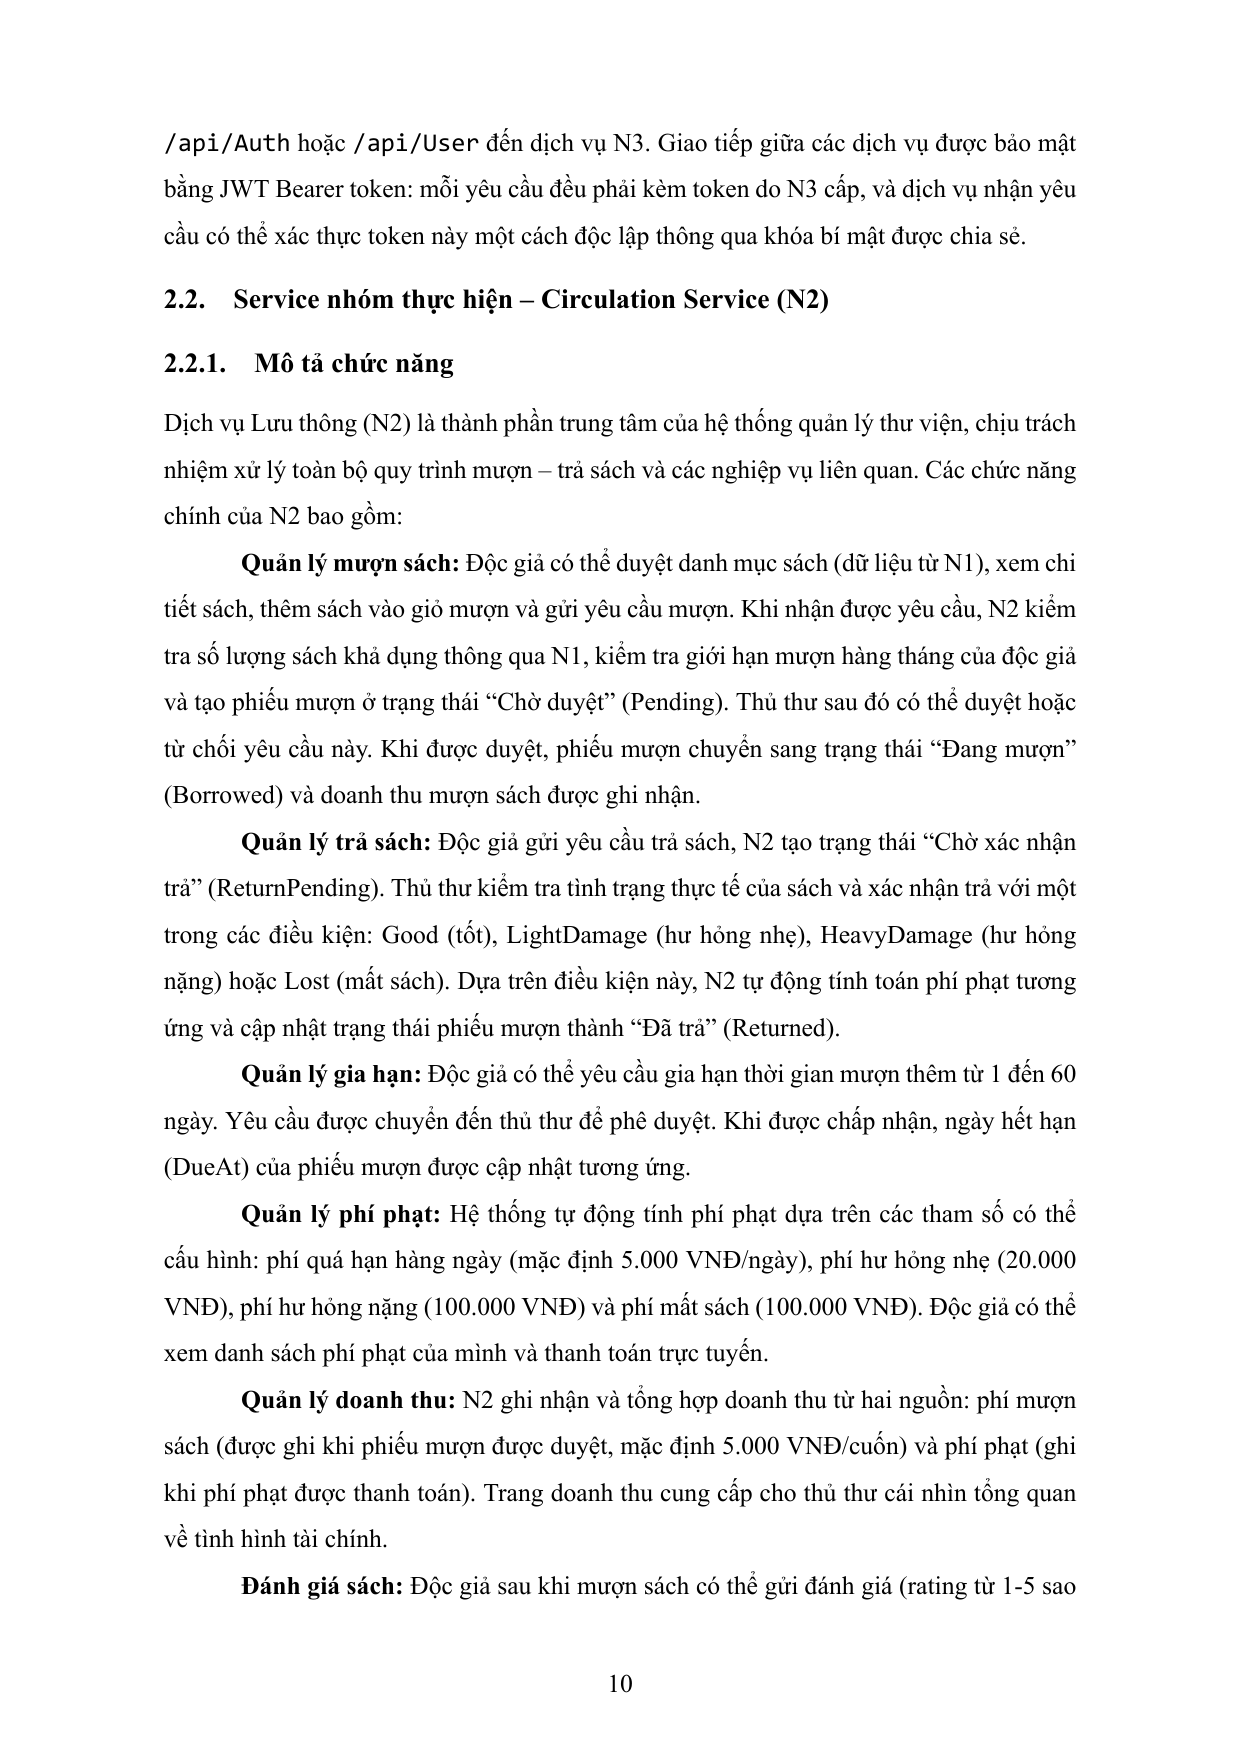
\includegraphics[width=0.98\textwidth]{figures/fig-23-23.png}
\caption{H?nh ?nh/s? ?? tr?ch t? b?o c?o g?c, trang 23}
\end{figure}
\clearpage
\begin{figure}[H]
\centering
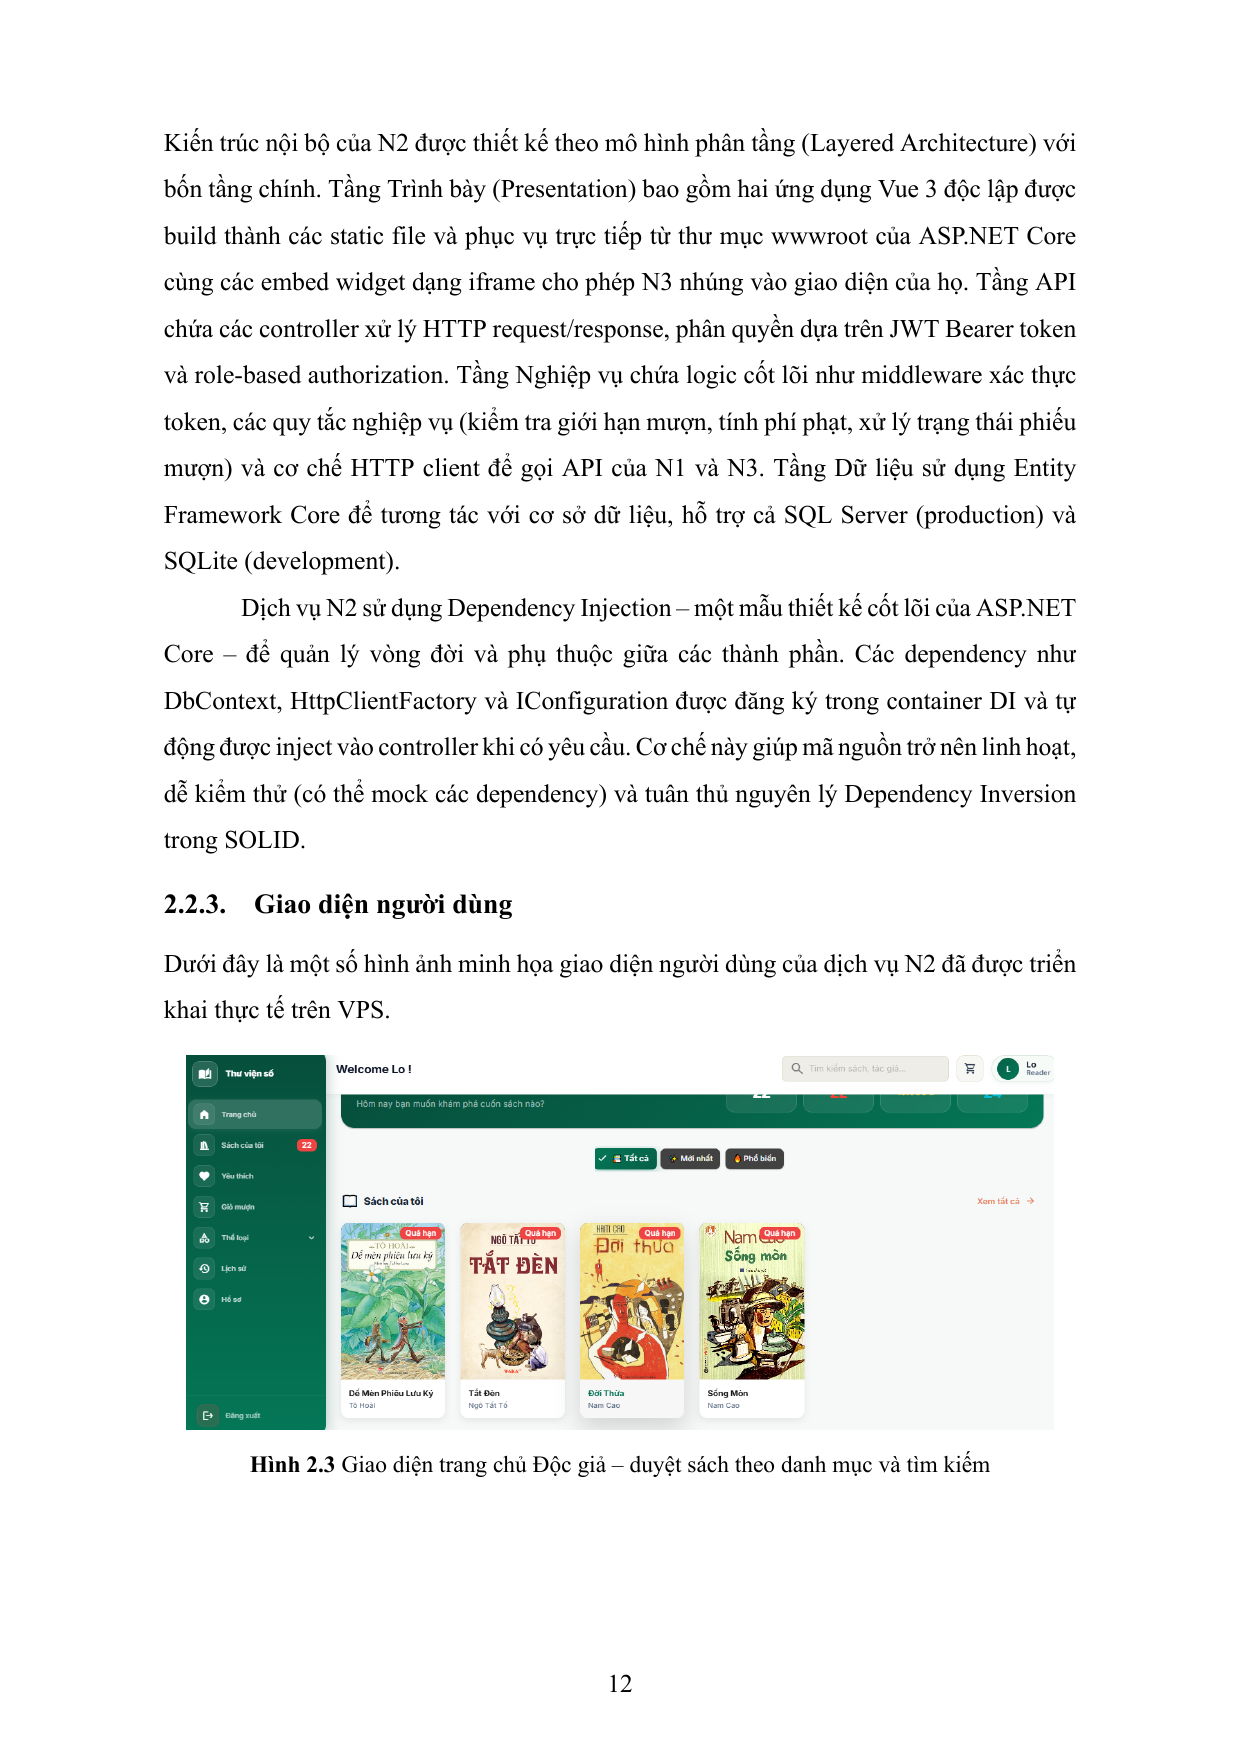
\includegraphics[width=0.98\textwidth]{figures/fig-25-25.png}
\caption{H?nh ?nh/s? ?? tr?ch t? b?o c?o g?c, trang 25}
\end{figure}
\clearpage
\begin{figure}[H]
\centering
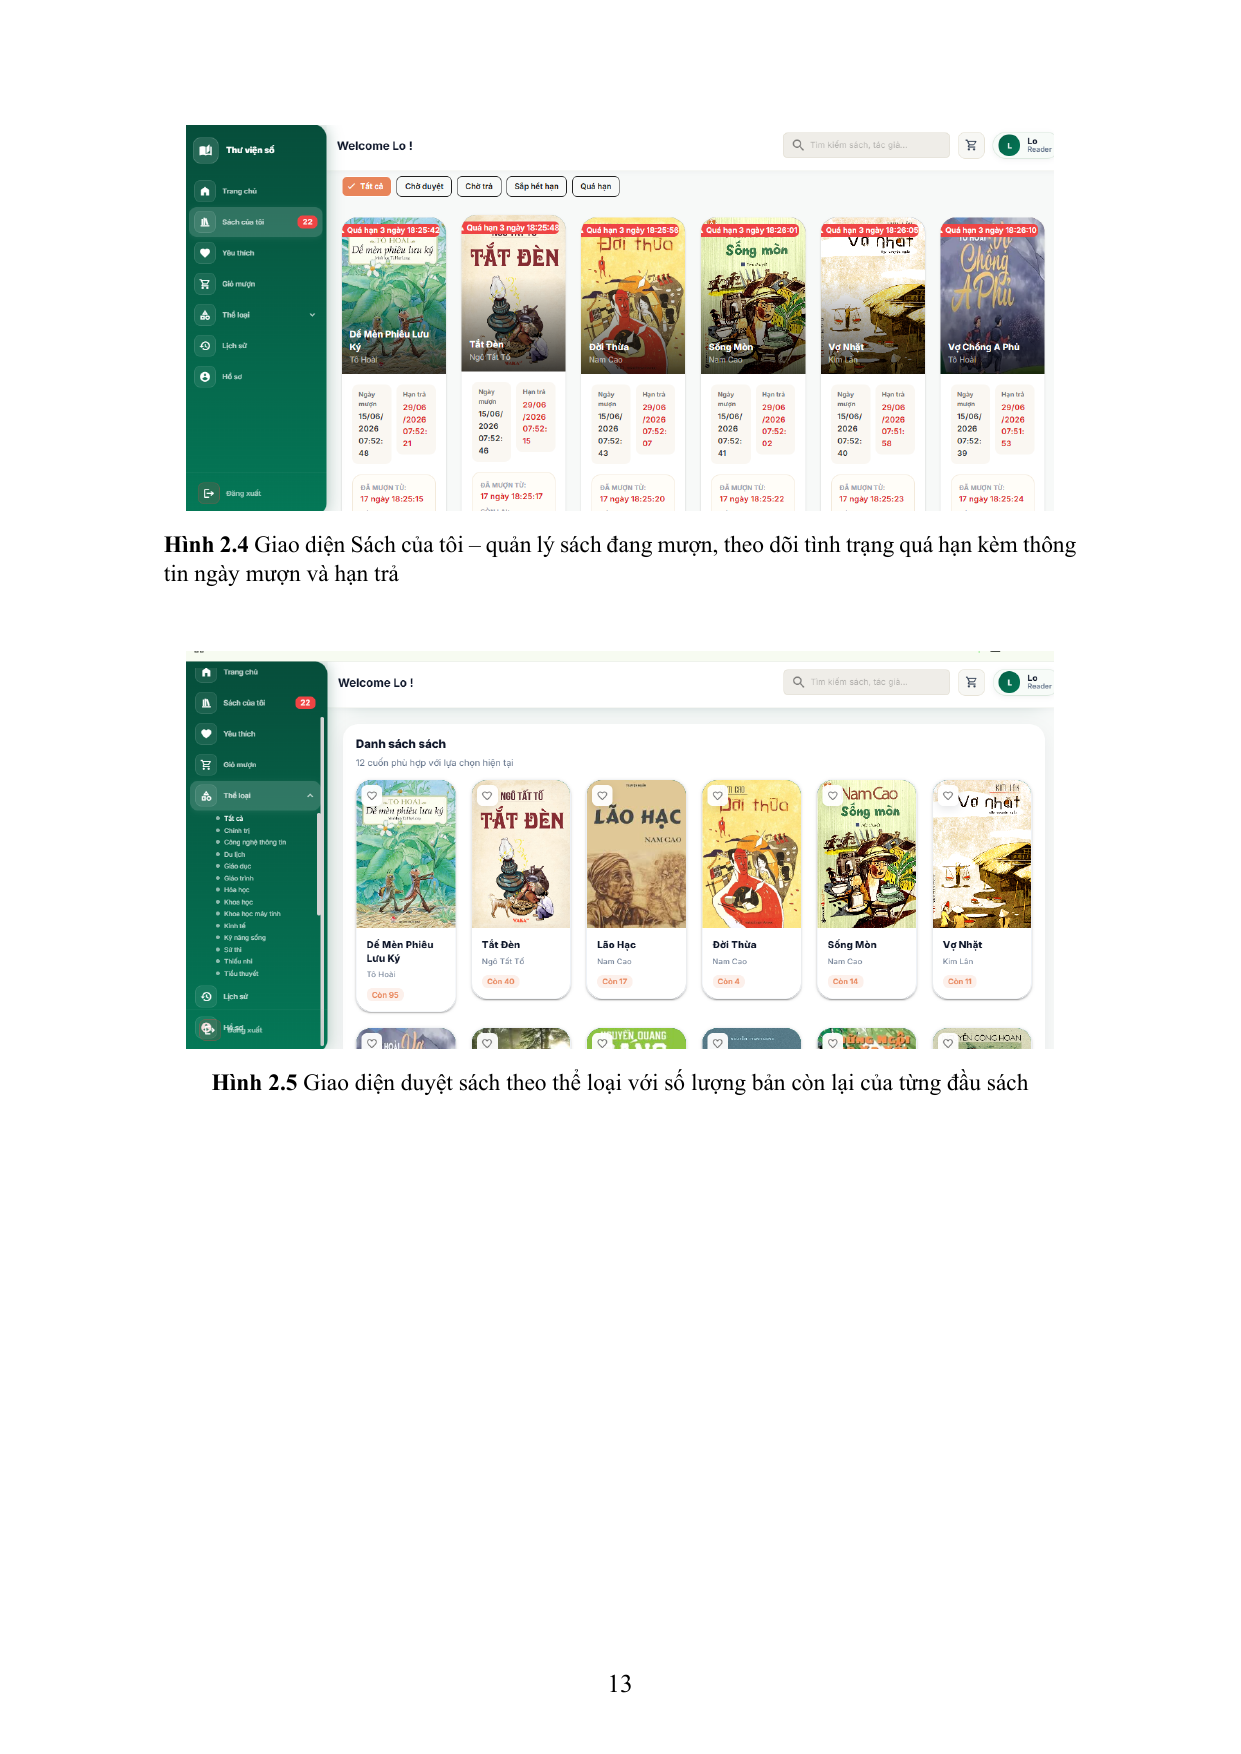
\includegraphics[width=0.98\textwidth]{figures/fig-26-26.png}
\caption{H?nh ?nh/s? ?? tr?ch t? b?o c?o g?c, trang 26}
\end{figure}
\clearpage
\begin{figure}[H]
\centering
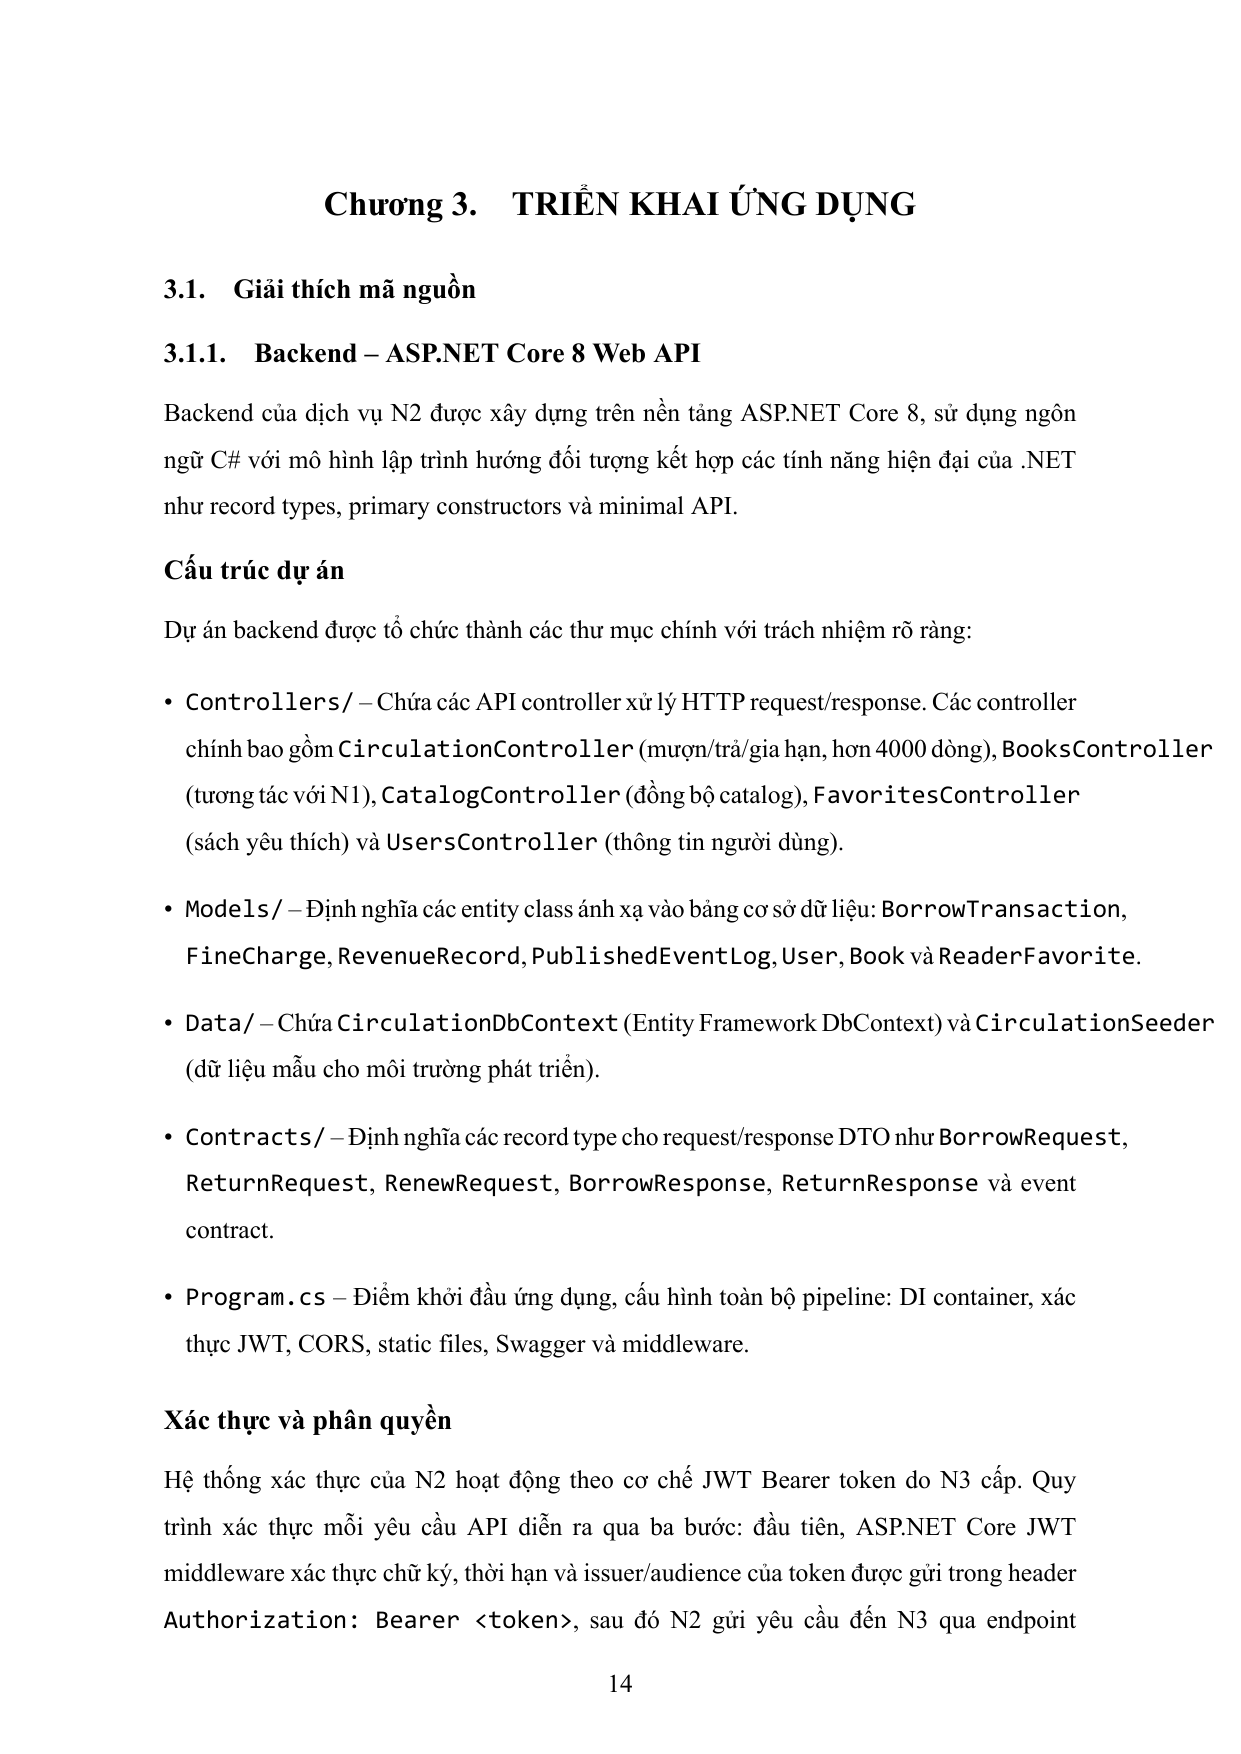
\includegraphics[width=0.98\textwidth]{figures/fig-27-27.png}
\caption{H?nh ?nh/s? ?? tr?ch t? b?o c?o g?c, trang 27}
\end{figure}
\clearpage
